\documentclass[12pt]{article}\usepackage[]{graphicx}\usepackage[]{color}
%% maxwidth is the original width if it is less than linewidth
%% otherwise use linewidth (to make sure the graphics do not exceed the margin)
\makeatletter
\def\maxwidth{ %
  \ifdim\Gin@nat@width>\linewidth
    \linewidth
  \else
    \Gin@nat@width
  \fi
}
\makeatother

\definecolor{fgcolor}{rgb}{0.345, 0.345, 0.345}
\newcommand{\hlnum}[1]{\textcolor[rgb]{0.686,0.059,0.569}{#1}}%
\newcommand{\hlstr}[1]{\textcolor[rgb]{0.192,0.494,0.8}{#1}}%
\newcommand{\hlcom}[1]{\textcolor[rgb]{0.678,0.584,0.686}{\textit{#1}}}%
\newcommand{\hlopt}[1]{\textcolor[rgb]{0,0,0}{#1}}%
\newcommand{\hlstd}[1]{\textcolor[rgb]{0.345,0.345,0.345}{#1}}%
\newcommand{\hlkwa}[1]{\textcolor[rgb]{0.161,0.373,0.58}{\textbf{#1}}}%
\newcommand{\hlkwb}[1]{\textcolor[rgb]{0.69,0.353,0.396}{#1}}%
\newcommand{\hlkwc}[1]{\textcolor[rgb]{0.333,0.667,0.333}{#1}}%
\newcommand{\hlkwd}[1]{\textcolor[rgb]{0.737,0.353,0.396}{\textbf{#1}}}%

\usepackage{framed}
\makeatletter
\newenvironment{kframe}{%
 \def\at@end@of@kframe{}%
 \ifinner\ifhmode%
  \def\at@end@of@kframe{\end{minipage}}%
  \begin{minipage}{\columnwidth}%
 \fi\fi%
 \def\FrameCommand##1{\hskip\@totalleftmargin \hskip-\fboxsep
 \colorbox{shadecolor}{##1}\hskip-\fboxsep
     % There is no \\@totalrightmargin, so:
     \hskip-\linewidth \hskip-\@totalleftmargin \hskip\columnwidth}%
 \MakeFramed {\advance\hsize-\width
   \@totalleftmargin\z@ \linewidth\hsize
   \@setminipage}}%
 {\par\unskip\endMakeFramed%
 \at@end@of@kframe}
\makeatother

\definecolor{shadecolor}{rgb}{.97, .97, .97}
\definecolor{messagecolor}{rgb}{0, 0, 0}
\definecolor{warningcolor}{rgb}{1, 0, 1}
\definecolor{errorcolor}{rgb}{1, 0, 0}
\newenvironment{knitrout}{}{} % an empty environment to be redefined in TeX

\usepackage{alltt}
\usepackage[T1]{fontenc}
\usepackage{garamondx}
\usepackage[garamondx,cmbraces]{newtxmath}
\usepackage[backend=biber]{biblatex}
\usepackage{fullpage}
\usepackage{array}
\usepackage{multirow}
\usepackage{setspace}
\usepackage{cleveref}

\addbibresource{papers.bib}
\IfFileExists{upquote.sty}{\usepackage{upquote}}{}
\begin{document}
\onehalfspacing

\newcommand{\tablepath}{../tables}
\graphicspath{{../figures/}}

\title{Reconstructing contact network parameters from viral phylogenies}
\author{Rosemary M. McCloskey, Richard H. Liang, and Art F.Y. Poon}
\abstract{Models of the spread of disease in a population often make the simplifying
assumption that the population is homogeneously mixed, or is divided into
homogeneously mixed compartments. However, human populations have complex
structures formed by social contacts, which can have a significant influence on
the rate of epidemic spread. Contact network models capture this structure by
explicitly representing each contact that could possibly lead to a
transmission. We developed a method based on approximate Bayesian computation
(ABC) for estimating structural parameters of the contact network underlying an
observed viral phylogeny. The method combines adaptive sequential Monte Carlo
for ABC, Gillespie simulation for propagating epidemics though networks, and a
kernel-based tree similarity score. We used the method to fit the
Barab\'{a}si-Albert network model to simulated transmission trees and applied
it to viral phylogenies estimated from six real-world HIV sequence datasets. On
simulated data, we found that the preferential attachment power and the number
of infected nodes in the network can often be accurately estimated. On the
other hand, the mean degree of the network, as well as the total number of
nodes, appeared to be weakly or non-identifiable with ABC. We observed
substantial heterogeneity in the parameter estimates on real datasets, with
point estimates for the preferential attachment power ranging from 0.06 to
1.05. These results underscore the importance of considering contact structures
when performing phylodynamic inference. Our method offers the potential to
quantitatively investigate the contact network structure underlying viral
epidemics.
}



\maketitle

\section{Introduction}

When an infectious disease spreads through a population, transmissions are
generally more likely to occur between certain pairs of individuals. Such pairs
must have a particular mode of contact with one another, which varies with the
mode of transmission of the disease. For airborne pathogens, physical proximity
may be sufficient, while for sexually transmitted diseases, sexual or in some
cases blood-to-blood contact is required. The population together with the set
of links between individuals along which transmission can occur is called the
contact network~\autocite{klovdahl1985social, morris1993epidemiology}. The
structure of the contact network underlying an epidemic can profoundly impact
the speed and pattern of the epidemic's expansion. Network structure can
influence the prevalence trajectory~\autocite{o2011contact} and epidemic
threshold~\autocite{barthelemy2005dynamical}, in turn affecting the estimates of
quantities such as effective population size~\autocite{goodreau2006assessing}.
From a public health perspective, contact networks have been explored as tools
for curtailing epidemic spread, by way of interventions targeted to
well-connected nodes~\autocite{wang2015targeting}. True contact networks are a
challenging type of data to collect, requiring extensive epidemiological
investigation~\autocite{welch2011statistical}.

Viral sequence data, on the other hand, has become relatively inexpensive and
straightforward to collect on a population level. Due to the high mutation rate
of RNA viruses, epidemiological processes impact the course of viral evolution,
thereby shaping the inter-host viral
phylogeny~\autocite{drummond2003measurably}. The term ``phylodynamics'' was
coined to describe this interaction, as well as the growing family of inference
methods to estimate epidemiological parameters from viral
phylogenies~\autocite{grenfell2004unifying}. These methods have revealed
diverse properties of local viral outbreaks, from basic reproductive
number~\autocite{stadler2012estimating}, to the degree of
clustering~\autocite{hughes2009molecular}, to the elevated transmission risk
during acute infection~\autocite{volz2012simple}. On the other hand, although
sophisticated methods have been developed for fitting complex population
genetic models to phylogenies~\autocite{rasmussen2014phylodynamic}, inference
of structural network parameters has to date been limited. However, it has been
shown that network structure has a tangible impact on phylogeny
shape~\autocite{leventhal2012inferring, colijn2014phylogenetic,
goodreau2006assessing, robinson2013dynamics, villandre2016assessment},
suggesting that such statistical inference might be
possible~\autocite{welch2011statistical}.

Survey-based studies of sexual networks~\autocite{liljeros2001web,
schneeberger2004scale, colgate1989risk} have found that these networks tend to
have a degree distribution which follows a power law \autocite[although there has
been some disagreement, see][]{handcock2004likelihood}. That is, the number of
nodes of degree $k$ is proportional to $k^{-\gamma}$ for some constant
$\gamma$. These networks are also creferred to as ``scale-free''. One process by
which scale-free networks can be generated is pcreferential attachment, where
nodes with a high number of contacts attract new connections at an elevated
rate. The first contact network model incorporating pcreferential attachment was
introduced by \textcite{barabasi1999emergence}, and is now creferred to as the
Barab\'asi-Albert (BA) model. Under this model, networks are formed by
iteratively adding nodes with $m$ new edges each. In the most commonly studied
formulation, these new edges are joined to existing nodes of degree $k$ with
probability proportional to $k$, so that nodes of high degree tend to attract
more connections. \citeauthor{barabasi1999emergence} suggested an extension
where the probability of attaching to a node of degree $k$ is $k^\alpha$ for
some non-negative constant $\alpha$, and we use this extension here.

Previous work offers precedent for the possibility of statistical inference of
structural network parameters. \textcite{britton2002bayesian} develop a Bayesian
approach to estimate the edge density in an Erd\H{o}s-R\'enyi
network~\autocite{erdos1960evolution} given observed infection dates, and
optionally recovery dates. Their approach was later extended by
\textcite{groendyke2011bayesian} and applied to a much larger data set of 188
individuals. \textcite{volz2007susceptible, volz2008sir} developed differential
equations describing the spread of a susceptible-infected (SI) epidemic on
static and dynamic contact networks with several degree distributions, which
could in principle be used for inference if observed incidence trajectories
were available. \textcite{brown2011transmission} analysed the degree distribution
of an approximate transmission network, estimated based on genetic similarity
and estimated times of infection, relating 60\% of HIV-infected men who have
sex with men (MSM) in the United Kingdom. The transmission network is a
subgraph of the contact network which includes only those edges which have
already led to a new infection. The authors found that a Waring distribution,
which is produced by a more sophisticated pcreferential attachment model, was a
good fit to their estimated network. 

Standard methods of model fitting involve calculation of the likelihood of
observed data under the model. In maximum likelihood estimation, a quantity
proportional to the likelihood is optimized, often through a standard
multi-dimensional numerical optimization procedure. Bayesian methods integrate
prior information by optimizing the posterior probability instead. To avoid
calculation of a normalizing constant, Bayesian inference is often performed
using Markov chain Monte Carlo (MCMC), which uses likelihood \emph{ratios} in
which the normalizing constants cancel out. Unfortunately, it is generally
difficult to explicitly calculate the likelihood of an observed transmission
tree under a contact network model, even up to a normalizing constant. To do
so, it would be necessary to integrate over all possible networks, and also
over all possible labellings of the internal nodes of the transmission tree.
While it is not known (to us) whether such integration is tractable, a simpler
alternative is offered by likelihood-free methods, namely approximate Bayesian
computation (ABC). ABC leverages the fact that, although calculating the
likelihood may be impractical, generating simulated datasets according to a
model is often straightforward. If our model fits the data well, the simulated
data it produces should be similar to the observed data. More formally, if $D$
is the observed data, the posterior distribution $f(\theta \mid D)$ on model
parameters $\theta$ is replaced as the target of statistical inference by
$f(\theta \mid \rho(\hat{D}, D) < \varepsilon)$, where $\rho$ is a distance
function, $\hat{D}$ is a simulated dataset according to $\theta$, and
$\varepsilon$ is a small tolerance~\autocite{sunnaaker2013approximate}. In the
specific case when $\rho$ is a kernel function, the approach is known as
kernel-ABC~\autocite{nakagome2013kernel, poon2015phylodynamic}.

Here, we develop a method using kernel-ABC to estimate the parameters of
contact network models from observed phylogenetic data. The distance function
we use is the tree kernel developed by \textcite{poon2013mapping}, which computes
a weighted dot product of the trees' representations in the space of all
possible subset trees. We apply the method to investigate the parameters of the
BA network model on a variety of simulated and real datasets. Our results show
that some network parameters can be inferred with reasonable accuracy, while
others have a minimal detectable impact on tree shape and thecrefore cannot be
estimated accurately. We also find that these parameters can vary considerably
between real epidemics from different settings.

\section{Methods}

\subsection{\textit{Netabc}: phylogenetic inference of contact network
parameters with kernel-ABC}

We have developed a kernel-ABC-based method to perform statistical inference of
contact network parameters from a transmission tree estimated from an observed
viral phylogeny. We implemented the adaptive sequential Monte Carlo (SMC)
algorithm for ABC developed by \textcite{del2012adaptive}. The SMC algorithm
keeps track of a population of parameter ``particles'', which are initially
sampled from the parameters' joint prior distribution. Several datasets are
simulated under the model of interest for each of the particles. In this case,
the datasets are transmission trees, which are generated by a two-step process.
First, a contact network is simulated according to the network model being fit.
Second, a transmission tree is simulated over that network with a Gillespie
simulation algorithm~\autocite{gillespie1976general}, in the same fashion as
several previous studies \autocite[\textit{e.g.}][]{robinson2013dynamics,
leventhal2012inferring}. The particles are weighted according to the similarity
between their associated simulated trees and the observed tree. To quantify
this similarity, we used the tree kernel developed by
\textcite{poon2013mapping}. Particles are iteratively perturbed by applying a
Metropolis-Hastings kernel and, if the move is accepted, simulating new
datasets under the new parameters. When a particle's weight drops to zero,
because its simulated trees are too dissimilar to the observed tree, the
particle is dropped from the population, and eventually replaced by a resampled
particle with a higher weight. As the algorithm progresses, the population
converges to a Monte Carlo approximation of the ABC target distribution, which
is assumed to approximate the desired posterior~\autocite{del2012adaptive,
sunnaaker2013approximate}. A computer program implementing our method is freely
available at \url{https://github.com/rmcclosk/netabc} (last accessed April 3,
2016).

To check that our implementation of Gillespie simulation was correct, we
reproduced Figure 1A of \textcite{leventhal2012inferring} (our
\cref{fig:leventhal}), which plots the unbalancedness of transmission trees
simulated over four network models at various levels of pathogen
transmissibility. Our implementation of adaptive ABC-SMC was tested by applying
it to the same mixture of Gaussians used by \citeauthor{del2012adaptive} to
demonstrate their method (originally used by~\textcite{sisson2007sequential}).
We were able to obtain a close approximation to the function (see
\cref{fig:smctest}), and attained the stopping condition used by the authors in
a comparable number of steps. 

Nodes in our networks followed simple SI dynamics, meaning that they became
infected at a rate proportional to their number of infected neighbours, and
never recovered. For all analyses, the transmission trees' branch lengths were
scaled by dividing by their mean. We used the \textit{igraph} library's
implementation of the BA model~\autocite{csardi2006igraph} to generate the
graphs. The analyses were run on Westgrid (\url{https://www.westgrid.ca/}) and
a local computer cluster.

\subsection{Kernel classifiers}
  
We used the phylogenetic kernel developed by \textcite{poon2013mapping} to test
whether the parameters of the BA model had an effect on tree shape. 100
networks were simulated under each of three different values of $\alpha$: 0.5,
1.0, and 1.5 (300 networks total). The other parameters were fixed to the
following values: $N$ = 5000, $I$ = 1000, and $m$ = 2. A transmission tree with
500 tips was simulated over each network (300 transmission trees total). The
300 trees were compared pairwise with the tree kernel to form a $300 \times
300$ kernel matrix. The kernel meta-parameters $\lambda$ (the ``decay
factor''), and $\sigma$ (the ``radial basis function
variance'')~\autocite[see][]{poon2013mapping}, were set to 0.3 and 4 respectively.
We constructed a kSVR classifier for $\alpha$ using the \textit{kernlab}
package~\autocite{zeileis2004kernlab}, and evaluated its accuracy with 1000
two-fold cross-validations.
  
Three similar experiments were performed for the other BA model parameters (one
experiment per parameter). $m$ was varied between 2, 3, and 4; $I$ between 500,
1000, and 2000; and $N$ between 3000, 5000, and 8000. The parameters not being
tested were fixed at the values $N$ = 5000, $I$ = 1000, $m$ = 2, and $\alpha$ =
1. Thus, we performed a total of four kSVR cross-validations, one for each of
the BA model parameters $\alpha$, $I$, $m$, and $N$. We repeated these four
cross-validations with different values of $\lambda$ (0.2, 0.3, and 0.4) and
$\sigma$ ($2^{-3}$, $2^{-2}$, \ldots, $2^3$), as well as on trees with
differing numbers of tips (100, 500, and 1000) and in epidemics of differing
size (500, 1000, and 2000). The combination of the number of sampled
individuals (\textit{i.e.} the number of tips) and the epidemic size
(\textit{i.e.} $I$) will be creferred to as an ``epidemic scenario''. When
evaluating the classifier for $I$, we did not consider trees with 1000 tips,
because one of the tested $I$ values was 500, and the number of tips cannot be
larger than $I$.
  
For each of the four parameters, we also tested a linear regression against
Sackin's index~\autocite{shao1990tree} and an ordinary SVR based on the normalized
lineages-through-time (nLTT) statistic~\autocite{janzen2015approximate}.
  
\subsection{ABC simulations}
  
We simulated three transmission trees, each with 500 tips, under every element
of the Cartesian product of these parameter values: $N$ = 5000, $I$ =
\{1000, 2000\}, $m$ = \{2, 3, 4\}, and $\alpha$ = \{0.0, 0.5, 1,
1.5\}. This produced a total of 24 parameter combinations $\times$ three trees
per combination = 72 trees total. The adaptive ABC algorithm was applied to
each tree with these priors: $m \sim$ DiscreteUniform(1, 5), $\alpha \sim$
Uniform(0, 2), and $(N, I)$ jointly uniform on the region \{$500 \leq N \leq
15000$, $500 \leq I \leq 5000$, $I \leq N$\}. Proposals for $\alpha$, $N$, and
$I$ were Gaussian, while proposals for $m$ were Poisson. Following
\textcite{del2012adaptive} and \textcite{beaumont2009adaptive}, the variance of
all proposals was equal to the empirical variance of the particles.

The algorithm was run with 1000 particles, 5 simulated datasets per particle,
and the ``quality'' parameter controlling the decay rate of the tolerance
$\varepsilon$ set to 0.95. We used the same stopping criterion as
\citeauthor{del2012adaptive}, namely when the MCMC acceptance rate dropped
below 1.5\%. Point estimates for the parameters were obtained by taking the
highest point of an estimated kernel density on the final set of particles,
calculated using the \textit{density} function with the default parameters in
\textit{R}. Highest posterior density (HPD) intervals were calculated with the
\textit{HPDinterval} function from the \textit{R} package
\textit{coda}~\autocite{plummer2006coda}.
  
Two further analyses were performed to address potential sources of error. To
evaluate the effect of model misspecification in the case of heterogeneity
among nodes, we generated a network where half the nodes were attached with
power $\alpha$ = 0.5, and the other half with power $\alpha$ = 1.5. The other
parameters for this network were $N$ = 5000, $I$ = 1000, and $m$ = 2. To
investigate the effects of potential sampling bias, we simulated a transmission
tree where the tips were sampled in a peer-driven fashion, rather than at
random. That is, the probability to sample a node was twice as high if any of
that node's network peers had already been sampled. The parameters of this
network were $N$ = 5000, $I$ = 2000, $m$ = 2, and $\alpha$ = 0.5.
  
\subsection{Investigation of published data}
  
We applied our kernel-ABC method to several published HIV datasets. Because the
BA model generates networks with a single connected component, we
specifically searched for datasets which originated from existing clusters,
either phylogenetically or geographically defined. Characteristics of the
datasets we investigated are given in \cref{tab:data}.
  
\begin{table*}[!t]
  \centering
  \begin{tabular}{ccccc}
  Reference & Sequences ($n$) & Location & Risk group & Gene \\
  \hline
  \textcite{wang2015targeting} & 173 & Beijing, China & MSM & \textit{pol} \\
  \textcite{cuevas2009hiv} & 287 & Basque Country, Spain & mixed & \textit{pol} \\
  \textcite{novitsky2013phylogenetic} & \multirow{2}{*}{180} &
  \multirow{2}{*}{Mochudi, Botswana} & \multirow{2}{*}{HET} &
  \multirow{2}{*}{\textit{env}} \\ \textcite{novitsky2014impact} \\
  \textcite{li2015hiv} & 280 & Shanghai, China & MSM & \textit{pol} \\
  \textcite{niculescu2015recent} & 136 & Romania & IDU & \textit{pol} \\
  \hline
\end{tabular}

  \caption{Characteristics of published datasets investigated with kernel-ABC.
  Acronyms: MSM, men who have sex with men; IDU, injection drug users.}
  \label{tab:data}
\end{table*}

We downloaded all sequences associated with each study from GenBank. For the
\textcite{novitsky2014impact} data, each sequence was aligned pairwise to the HXB2
creference sequence (Genbank accession number K03455) and the hypervariable
regions were clipped out with \textit{BioPython} version
1.66+~\autocite{cock2009biopython}. Sequences were multiply aligned using
\textit{MUSCLE} version 3.8.31 \autocite{edgar2004muscle}, and alignments were
manually inspected with \textit{Seaview} version 4.4.2
\autocite{gouy2010seaview}. Phylogenies were constructed from the nucleotide
alignments by approximate maximum likelihood using \textit{FastTree2} version
2.1.7 with the generalized time-reversible model. Transmission trees were
estimated by rooting and time-scaling the phylogenies by root-to-tip
regression, using a modified version of Path-O-Gen (distributed as part of
BEAST~\autocite{drummond2007beast}) as described
previously~\autocite{poon2015phylodynamic}. 

Two of the datasets \autocite{li2015hiv,novitsky2014impact} were initially much
larger than the others, containing 1265 and 1299 sequences respectively. To
ensure that the analyses were comparable, we reduced these to a number of
sequences similar to the smaller datasets. For the \textcite{li2015hiv} data,
we detected a cluster of size 280 using a patristic distance cutoff of 0.02 as
described previously~\autocite{poon2015impact}. Only sequences within this
cluster were carried forward. For the \textcite{novitsky2014impact} data, no
large clusters were detected using the same cutoff, so we analysed a subtree of
size 180 chosen arbitrarily.

For all datasets, we used the priors $\alpha$ $\sim$ Uniform(0, 2) and $N$ and
$I$ jointly uniform on the region \{$n \leq N \leq 10000$, $n \leq I \leq
10000$, $I \leq N$\}, where $n$ is the number of tips in the tree. Since the
value $m = 1$ produces networks with no cycles, which we considered fairly
implausible, we ran one analysis with the prior $m \sim$ DiscreteUniform(1, 5),
and one with the prior $m \sim$ DiscreteUniform(2, 5). The other parameters to
the SMC algorithm were the same as used for the simulation experiments.


\section{Results}

\subsection{Kernel classifiers}



We investigated the parameters of the BA network
model~\autocite{barabasi1999emergence}. In addition to $m$ and $\alpha$ (see
Introduction), we considered $N$, which denotes the total number of nodes in
the network, and $I$, which is the number of infected nodes at which to stop
the simulation and sample the transmission tree. To examine the effect of these
parameters on tree shape, we simulated transmission trees under different
parameter values, calculated pairwise tree kernel scores between them, and
attempted to classify the trees using a kernel support vector machine (kSVR).
We also tested classifiers based on Sackin's index~\autocite{shao1990tree} and
the normalized lineages-through-time (nLTT)
statistic~\autocite{janzen2015approximate}. Accuracy of the kSVRs varied based
on the parameter being tested (\cref{fig:rsquared}, left). Classifiers based on
two other tree statistics, the nLTT and Sackin's index, generally exhibited
worse performance than the tree kernel, although the magnitude of the disparity
varied between the parameters (\cref{fig:rsquared}, centre and right). The
results were largely robust to variations in the tree kernel meta-parameters
$\lambda$ and $\sigma$ (\cref{fig:alphacrossv,fig:mcrossv,fig:Ncrossv,fig:Icrossv}).

When classifying $\alpha$, the kernel-SVR classifier had an average $R^2$ of 
    0.92,
compared to 
    0.56
for the nLTT-based SVR, and
    0.75
for the linear regression against Sackin's index. There was little variation
about the mean for different tree and epidemic sizes. No classifier could
accurately identify the $m$ parameter in any epidemic scenario, with average
$R^2$ values of 
  0.12 for kSVR,
  0.01 for the nLTT, and
  0.06
for Sackin's index. Again, there was little variation in accuracy between
epidemic scenarios, although the accuracy of the kSVR was slightly higher
on 1000-tip trees (\cref{fig:rsquared}, left).

The accuracy of classifiers for $I$ varied significantly with the number of
tips in the tree. For 100-tip trees, the average $R^2$ values were
  0.7,
  0.55, and
  0.02
for the tree kernel, nLTT, and Sackin's index respectively. For 500-tip
trees, the values increased to
  0.93,
  0.83, and
  0.07.
Finally, the performance of classifiers for $N$ depended heavily on the
epidemic scenario. The $R^2$ of the kSVR classifier ranged from
  0.08
for the smallest epidemic and smallest sample size, to
  0.82
for the largest. Likewise, $R^2$ for the nLTT-based SVR ranged from 
  0.01
to
  0.54.
Sackin's index did not accurately classify $N$ in any scenario, with an average
$R^2$ of
  0.03
and little variation between scenarios.

\begin{figure*}[ht]
  \centering
  \includegraphics[width=\textwidth]{kernel-rsquared.eps}
  \vspace{6pt}
  \caption{
      Cross-validation accuracy of kernel-SVR classifier (left), SVR classifier
      using nLTT (centre), and linear regression using Sackin's index
      (right) for BA model parameters. Kernel meta-parameters were set to
      $\lambda = 0.3$ and $\sigma = 4$. Each point was calculated based on 300
      simulated transmission trees over networks with three different values of
      the parameter being tested. Vertical lines are empirical 95\% confidence
      intervals based on 1000 two-fold cross-validations.
  }
  \label{fig:rsquared}
\end{figure*}

\subsection{ABC simulations}

%<<point_est, include=FALSE>>=
%    f <- Sys.glob("../../simulations/abc-pa-free-m/point-estimate/*")
%    d <- fread(f)
%    d[,m := floor(m)]
%    d[,alpha_error := abs(true_alpha - alpha)]
%    d[,N_error := abs(true_N - N)]
%    d[,I_error := abs(true_I - I)]
%    d[,m_error := abs(true_m - m)]
%
%    alpha.av <- anova(lm(alpha_error ~ factor(true_alpha) + factor(true_m) + factor(true_I), d))
%    m.av <- anova(lm(m_error ~ factor(true_alpha) + factor(true_m) + factor(true_I), d))
%    N.av <- anova(lm(N_error ~ factor(true_alpha) + factor(true_m) + factor(true_I), d))
%    I.av <- anova(lm(I_error ~ factor(true_alpha) + factor(true_m) + factor(true_I), d))
%
%    m.tbl <- d[,prop.table(table(m_error))]
%    zero.alpha.test <- wilcox.test(d[true_alpha == 0, alpha_error], 
%                                   d[true_alpha != 0, alpha_error])
%    alpha.I.test <- wilcox.test(d[true_alpha < 1, I_error],
%                                d[true_alpha >= 1, I_error])
%    I.I.test <- wilcox.test(d[true_I == 1000, I_error],
%                            d[true_I == 2000, I_error])
%    alpha.m.test <- wilcox.test(d[true_alpha == 0 | true_alpha == 1, m_error],
%                                d[true_alpha == 0.5 | true_alpha == 1.5, m_error])
%    stopifnot(alpha.av["factor(true_m)", "Pr(>F)"] > 0.05)
%    stopifnot(alpha.av["factor(true_I)", "Pr(>F)"] > 0.05)
%    stopifnot(I.I.test$p.value < 1e-5)
%    stopifnot(I.av["factor(true_m)", "Pr(>F)"] > 0.05)
%    stopifnot(m.av["factor(true_m)", "Pr(>F)"] > 0.05)
%    stopifnot(m.av["factor(true_I)", "Pr(>F)"] > 0.05)
%    stopifnot(min(N.av[1:3,"Pr(>F)"]) > 0.05)
%@

\Cref{fig:abcpt} shows maximum \textit{a posteriori} (MAP) point
estimates of the BA model parameters obtained with kernel-ABC on simulated
data. The estimates shown correspond only to the simulations where the $m$
parameter was set to 2, however the results for $m = 3$ and $m = 4$ were
similar (\cref{fig:abcptm3,fig:abcptm4}). Average boundaries of 95\% HPD
intervals are given in \cref{tab:abchpd}.

The accuracy of the parameter estimates obtained with kernel-ABC
paralleled the results from the kSVR classifier. Of the four parameters,
$\alpha$ was the most accurately estimated, with point estimates having a
median [IQR] absolute error of 
%    d[,round(median(alpha_error), 2)] 
%    [d[,round(quantile(alpha_error, 0.25), 2)] - 
%    d[,round(quantile(alpha_error, 0.75), 2)]].
The errors when the true value of $\alpha$ was zero were significantly greater
than those for the other values 
%    (Wilcoxon rank-sum test, $p$ = $latexSN(round(zero.alpha.test$p.value, 4))$),
but did not vary across the true values of the other parameters (one-way
ANOVA). Estimates for $I$ were also relatively accurate, with point estimate
errors of
%    d[,round(median(I_error))] 
%    [d[,round(quantile(I_error, 0.25))] - 
%    d[,round(quantile(I_error, 0.75))]].
These errors were significantly higher when the true value of $\alpha$ was
at least 1
%    (Wilcoxon rank-sum test, $p$ = $latexSN(round(alpha.I.test$p.value, 4))$)
and when the true value of $I$ was 2000 ($p < 10^{-5}$). The true value of $m$
did not affect the estimates of $I$ (one-way ANOVA).

The $m$ parameter was estimated correctly in only
%    as.integer(m.tbl[1] * 100) \%
of simulations. Oddly, the error in the estimated $m$ was higher for integer
values of $\alpha$ (\textit{i.e.}~0 and 1) than non-integer values 
%    (Wilcoxon rank-sum test, $p$ = round(alpha.m.test$p.value, 3)).
The true values of the other parameters did not significantly affect the
estimates of $m$ (both one-way ANOVA). Finally, the total number of nodes $N$
was consistently over-estimated by about a factor of two
%    (error d[,round(median(N_error))] 
%    [d[,round(quantile(N_error, 0.25))] - 
%     d[,round(quantile(N_error, 0.75))]]).
No parameters influenced the accuracy of the $N$ estimates (all one-way ANOVA).

\begin{figure*}[ht]
  \centering
  \includegraphics[width=\textwidth]{abc-point-estimate-m2.eps}
  \vspace{6pt}
  \caption{
    Point estimates of BA model parameters obtained by running kernel-ABC
    on simulated phylogenies without training, for simulations with $m = 2$.
    Dotted lines indicate true values, and limits of the $y$-axes are regions
    of uniform prior density. (A) Estimates for $\alpha$ and $I$ against their
    true values in simulations. (B) Estimates for $m$ and $N$, which were held
    fixed in these simulations, against true values of $\alpha$.
  }
  \label{fig:abcpt}
\end{figure*}

\begin{table*}[ht]
  \centering
  % latex table generated in R 3.2.3 by xtable 1.8-2 package
% Fri Jun 17 12:51:45 2016
\begin{tabular}{lr>{\raggedleft\arraybackslash}p{2.5cm}>{\raggedleft\arraybackslash}p{2.5cm}>{\raggedleft\arraybackslash}p{2.5cm}}
  \hline
Parameter & True value & Mean point estimate & Mean HPD lower bound & Mean HPD upper bound \\ 
  \hline
$\alpha$ & 0.0 & 0.36 & 0.01 & 0.81 \\ 
   & 0.5 & 0.43 & 0.04 & 0.83 \\ 
   & 1.0 & 0.90 & 0.51 & 1.09 \\ 
   & 1.5 & 1.52 & 1.26 & 1.81 \\ 
  $I$ & 1000 & 1450 & 651 & 2592 \\ 
   & 2000 & 2622 & 1114 & 4080 \\ 
  $m$ & 2 & 2.96 & 2.00 & 5.00 \\ 
   & 3 & 3.04 & 2.04 & 4.96 \\ 
   & 4 & 3.17 & 1.88 & 5.00 \\ 
  $N$ & 5000 & 9041 & 2613 & 14659 \\ 
   \hline
\end{tabular}

  \caption{
      Average maximum \textit{a posteriori} point estimates and 95\% highest
      posterior density (HPD) interval widths for BA model parameter estimates
      obtained with kernel-ABC. Three transmission trees were simulated under
      each combination of the listed parameter values, and the parameters were
      estimated with kernel-ABC without training.
  }
  \label{tab:abchpd}
\end{table*}

The dispersion of the ABC approximation to the posterior also varied between
the parameters, with narrower HPD intervals for the parameters with more
accurate point estimates (\cref{tab:abchpd}). \Cref{fig:abcex} shows
the distributions for for one simulation (equivalent plots for all the
simulations can be found in Supplementary Figures TODO). HPD intervals around
$\alpha$ and $I$ were narrow relative to the region of nonzero prior density,
whereas the intervals for $m$ and $N$ were more widely dispersed.

\begin{figure*}[ht]
    \centering
  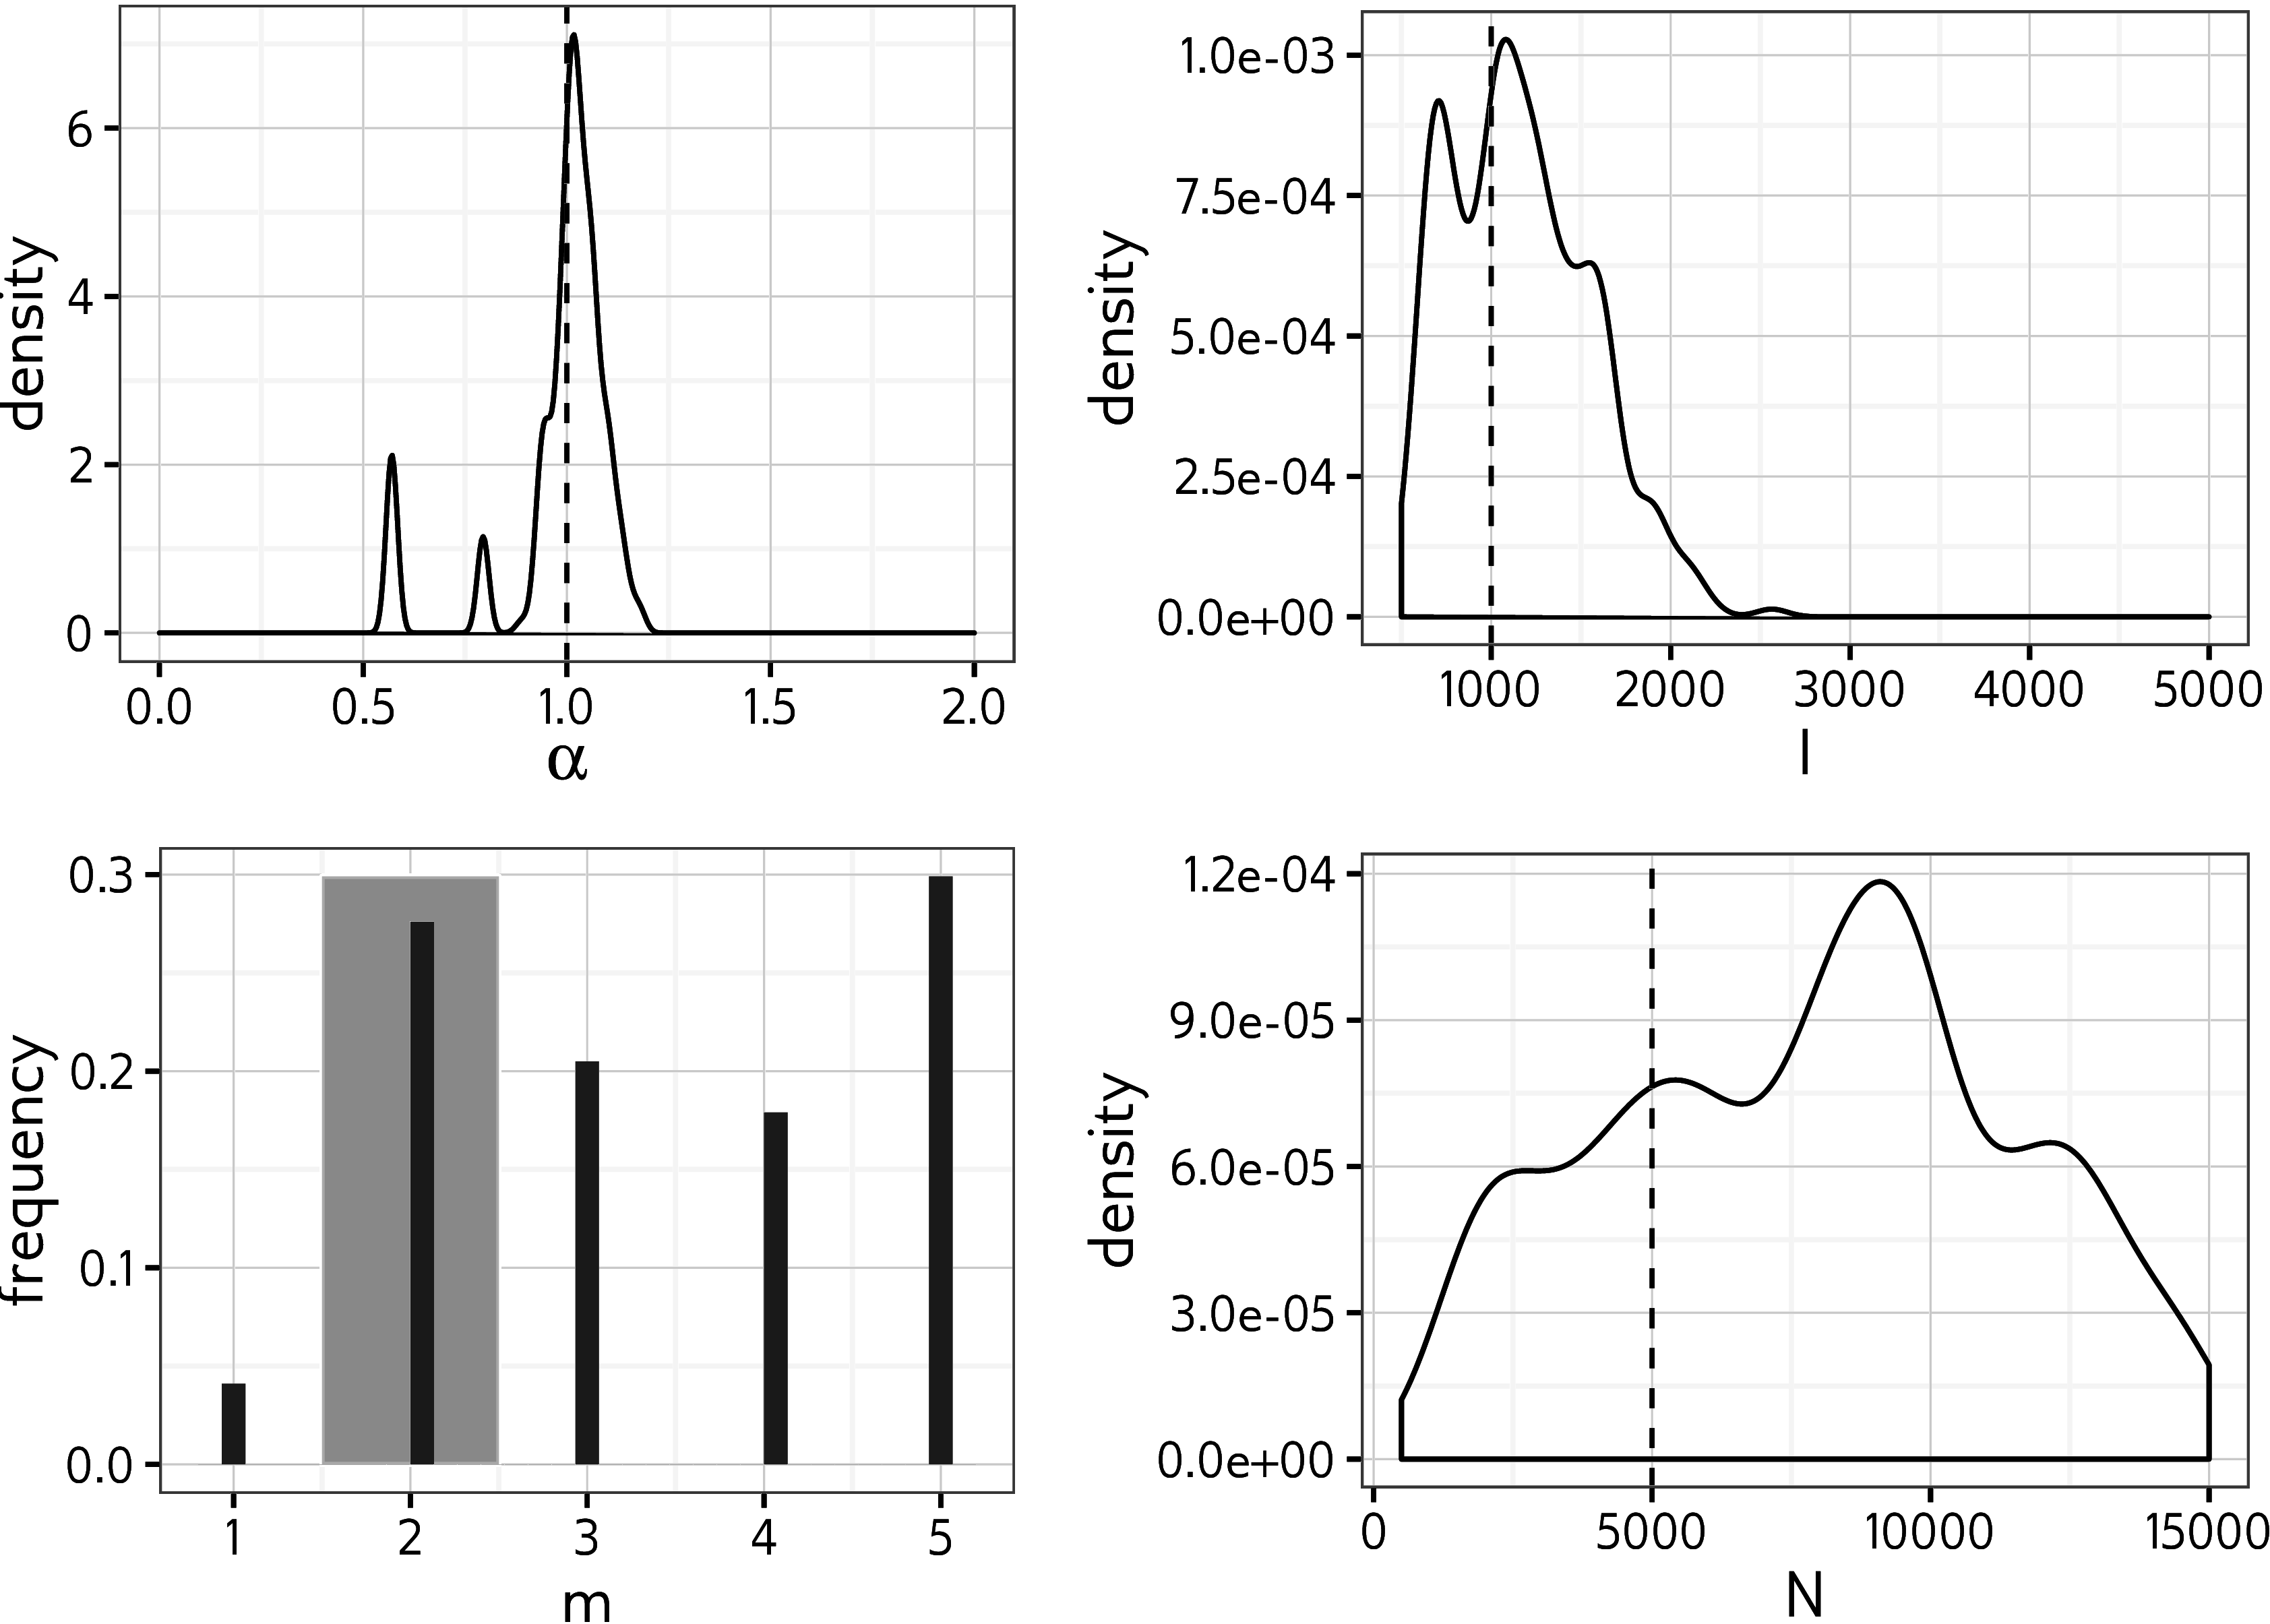
\includegraphics[width=\textwidth]{abc-posterior-example.eps}
  \vspace{6pt}
  \caption{
    Marginal posterior distributions of BA model parameters estimated
    with kernel-ABC for a single simulated transmission tree. Dotted
    lines and shaded polygon indicate true values.
  }
  \label{fig:abcex}
\end{figure*}



To test the effect of model misspecification, we simulated one network where
the nodes exhibited heterogeneous pcreferential attachment power (half 0.5, the
other half 1.5), with $m$ = 2, $N$ = 5000, and $I$ = 1000. The MAP [95\%
HPD] estimates for each parameter were: 
$\alpha$, 
  1.1 
  [0.6 -
   1.15];
$I$,
  1141 
  [662 -
   4455];
$m$,
  3 
  [2 -
   5];
$N$,
  12689 
  [3733-
   14977].
To test the effect of sampling bias, we sampled one transmission tree in a
peer-driven fashion, where the probability to sample a node was twice as high
if one of its peers had already been sampled. The parameters for this
experiment were $N$ = 5000, $m$ = 2, $\alpha$ = 0.5, and $I$ = 2000. The
estimated values were
$\alpha$, 
  0.36 
  [0.01 -
   0.63];
$I$,
  2392 
  [1419 -
   3767];
$m$,
  3 
  [2 -
   5];
$N$,
  8760 
  [2881 -
   14788].
Both of these results were in line with estimates obtained on other simulated
datasets (\cref{tab:abchpd}).

\subsection{Real data}



We applied kernel-ABC to five published HIV datasets (\cref{tab:data}),
and found substantial heterogeneity among the parameter estimates
(\cref{fig:abchpd,fig:abchpdm2}). Two of the
datasets~\autocite{niculescu2015recent, wang2015targeting} had estimated
$\alpha$ values near unity for the prior allowing $m = 1$ (MAP estimates
[95\% HPD] 
  1.05 
  [0.04 - 
   1.27]
and
  0.84 
  [0.01 -
   1.02] respectively).
The MAP estimates did not change appreciably when $m = 1$ was disallowed by the
prior, although the credible interval of the \textcite{niculescu2015recent}
data was narrower
  (0.04 - 
   1.27).
When $m = 1$ was permitted, the \textcite{li2015hiv, cuevas2009hiv} both had
low estimated $\alpha$ values
  (0.06 
  [0.01 - 
  0.73]
and
  0.19 
  [0.01 -
   0.8]). 
However, the MAP estimates increased when $m = 1$ was not permitted, although
the HPD intervals remained roughly the same
  (0.78 
  [0.02 - 
  0.94]
and
  0.59 
  [0.07 -
   0.95]).
The \textcite{novitsky2014impact} data had a fairly low estimated $\alpha$
for both priors on $m$
  (0.32 for $m \geq 1$;
   0.39 for $m \geq 2$).
However, the confidence interval was much wider when $m = 1$ was allowed
  ([0.04 -
    1.62] for $m \geq 1$ vs.
    0 -
    0.73 for $m \geq 2$).

For all the datasets except \citeauthor{novitsky2014impact}, estimated values
of $I$ were below 2000 when $m = 1$ was allowed, with relatively narrow HPD
intervals compared to the nonzero prior density region
  (\citeauthor{cuevas2009hiv}, 482 
  [293 -
   2111];
   \citeauthor{niculescu2015recent}, 307
  [136 - 
   2822];
  (\citeauthor{li2015hiv}, 1183 
  [413 -
   2897];
   \citeauthor{wang2015targeting}, 719
  [176 - 
   2114]).
The \citeauthor{novitsky2014impact} data was the outlier, with a very high
estimated $I$, and HPD interval spanning almost the entire prior region
  (7409 
  [187 -
   8819]).
The $I$ estimates and HPD intervals were generally robust to the choice of
prior on $m$, with slightly narrower HPD intervals (compare
\cref{fig:abchpd,fig:abchpdm2}).

The MAP estimate of $m$ was equal to 1 for all but the
\citeauthor{novitsky2014impact} data, when this value was allowed. However, the
upper bound of the HPD interval was different for each dataset
  (\citeauthor{niculescu2015recent}, 5;
   \citeauthor{wang2015targeting}, 4;
   \citeauthor{li2015hiv}, 1;
   \citeauthor{cuevas2009hiv}, 2).
When $m = 1$ was disallowed, the MAP for all datasets was either 2 or 3, with
HPD intervals spanning the entire prior region. The estimates for the total
number of nodes $N$ were largely uninformative for all samples, with almost all
MAP estimates greater than 5000 and HPD intervals spanning almost the entire
nonzero prior density region. The only exception was the \citeauthor{li2015hiv}
data, for which the MAP estimate was lower 
  (6973)
when $m = 1$ was allowed.

\begin{figure*}[ht]
  \centering
  \includegraphics{realdata-hpd}
  \vspace{8pt}
  \caption{
      Maximum \textit{a posteriori} point estimates and 95\% HPD intervals for
      parameters of the BA network model, fitted to five published HIV datasets
      with kernel-ABC.
  }
  \label{fig:abchpd}
\end{figure*}

\section{Discussion}

Contact networks can have a strong influence on epidemic progression, and are
potentially useful as a public health tool~\autocite{wang2015targeting,
little2014using}. Despite this, few methods exist for investigating contact
network parameters in a phylodynamic framework~\autocite{groendyke2011bayesian,
volz2008sir, brown2011transmission, leventhal2012inferring}. Kernel-ABC is a
model-agnostic method which can be used to investigate any quantity that
affects tree shape~\autocite{poon2015phylodynamic}. In this work, we developed a
kernel-ABC-based method to infer the parameters of a contact network model. The
method is general, and could be applied to any model from which contact
networks can be simulated. We demonstrated the method on the BA model,
which is a simple pcreferential attachment model giving rise to the power law
degree distributions commonly observed in real-world networks. 

By training a kernel-SVR classifier, we found that the $\alpha$ and $I$
parameters, representing pcreferential attachment power and number of infected
nodes, had a strong influence on tree shape. This was creflected in the relative
accuracy of the kernel-ABC estimates of these parameters. The total number of
nodes $N$ had a weak influence on tree shape, which was most prominent when the
epidemic size $I$ and number of sampled tips were both large. The $m$
parameter, representing the number of edges created in the network per vertex,
did not produce much variation in tree shape, resulting in in both poorly
performing classifiers and uninformative kernel-ABC estimates.

$N$ was almost always significantly over-estimated using kernel-ABC. Since the
prior on $N$ and $I$ is jointly uniform on a non-rectangular region ($I \leq
N$), there is more prior mass on high $N$ values. In retrospect, it is
unreasonable to expect good estimation of $N$, because adding more nodes to a
BA network does not change the edge density or overall shape. This can be
illustrated by imagining that we add a small number of nodes to a network after
the epidemic simulation has already been completed. It is possible that none of
these new nodes attains a connection to any infected node. Thus, running the
simulation again on the new, larger network could produce the exact same
transmission tree as before. We note also that our accurate estimates of $I$
may have been influenced by this prior, which places more mass on low $I$
values. However, the MAP estimate of $I$ was very high for the
\textcite{novitsky2013phylogenetic,novitsky2014impact} data, suggesting that a
strong enough signal in the data can overcome the prior.

As noted by \textcite{lintusaari2016identifiability}, uniform priors on model
parameters may translate to highly informative priors on quantities of
interest. We observed a non-linear relationship between the pcreferential
attachment power $\alpha$ and the power law exponent $\gamma$
(\cref{fig:gamma}). Thecrefore, placing a uniform prior on $\alpha$ between 0
and 2 is equivalent to placing an informative prior that $\gamma$ is close to
2. Thecrefore, if we were primarily interested in $\gamma$ rather than
$\alpha$, a more sensible choice of prior might have a shape similar to the
inverse of \cref{fig:gamma} and be bounded above by approximately $\alpha$ =
1.5. This would uniformly bound $\gamma$ in the region $2 \leq \gamma \leq 4$
commonly reported in the network literature~\autocite{liljeros2001web,
schneeberger2004scale, colgate1989risk, brown2011transmission}. We note however
that \textcite{jones2003assessment} estimated $\gamma$ values greater than
four, in one case as high as 17, for some datasets, indicating that a wider
range of permitted $\gamma$ values may be warranted.

Our investigation of published HIV datasets indicated heterogeneity in the
contact network structures underlying several distinct local epidemics. When
interpreting these results, we caution that the BA model is quite simple and
most likely misspecified for these data. In particular, the average degree of a
node in the network is equal to $2m$, and thecrefore is constrained to be a
multiple of 2. Furthermore, we considered the case $m = 1$, where the network
has no cycles, to be implausible and thecrefore assigned it zero prior
probability in one set of analyses. This forced the average degree to be at
least four, which may be unrealistically high for sexual networks. The fact
that the estimated values of $\alpha$ differed substatially for three datasets
depending on whether or not $m = 1$ was allowed by the prior is futher evidence
of this potential misspecification. However, we note that for two of the
datasets, the estimated values of $\alpha$ did not change much between priors,
and the estimates of $I$ were robust to the choice of prior for all datasets
studied. More sophisticated models, for example models incorporating
heterogeneity in node behaviour, are likely to provide a better fit to these
data.

With respect to the pcreferential attachment power $\alpha$, the five datasets
analysed fell into three categories (\cref{fig:abchpd}). First, we
estimated a pcreferential attachment power close to 1, indicating linear
pcreferential attachment, for the outbreaks studied by
\textcite{niculescu2015recent} and \textcite{wang2015targeting}. These values
were robust to specifying different priors for $m$. Both studies were of
populations in which we would expect a high degree of epidemiological
relatedness: \textcite{niculescu2015recent} studied a recent outbreak among
Romanian injection drug users (IDU), while \citeauthor{wang2015targeting}
sampled acutely infected MSM in Beijing, China. Both these are contexts in
which we would expect some of the assumptions of the BA model, such as a
connected network, relatively high mean degree, and pcreferential attachment
dynamics, to hold.

The remaining three datasets (\textcite{cuevas2009hiv, novitsky2014impact,
li2015hiv}) had estimated values of $\alpha$ below 0.5 when $m = 1$ was
included in the prior, but these were not robust to changing the prior to
exclude $m = 1$. For the \citeauthor{cuevas2009hiv} data, model
misspecification is likely partially responsible. While the authors found that
a large proportion of the samples were epidemiologically linked, these were
mainly in small local clusters rather than the single large component
postulated by the BA model. In addition, the mixed risk groups in the dataset
would be unlikely to significantly interact, further weakening any global
pcreferential attachment dynamics. The dataset studied by
\textcite{novitsky2014impact} originated from a densely sampled population
where the predominant risk factor was believed to be heterosexual exposure.
Although the MAP estimate of $\alpha$ was almost unchanged when the value $m =
1$ was excluded from the prior, the confidence interval shrank significantly.
For both priors, the estimated prevalence was extremely high, in fact higher
than the estimated HIV prevalence in the sampled region. The authors indicated
that the source of the samples was a town in close proximity to the country's
capital city, and suggested that there may have been a high degree of migration
and partner interchange between the two locations. It is possible that the
contact network underlying the subtree we investigated includes a much larger
group based in the capital city, which would explain the high estimate of $I$.
There is no clear explanation for the discrepancy between the two priors for
the \textcite{li2015hiv} data, as the subset we analyzed formed a phylogenetic
cluster and thecrefore was a good candidate for the BA model. However, nearly
all the posterior density was assigned to $m = 1$ when this value was allowed,
indicating that the network was more likely to have an acyclic tree structure.

In addition to the aforementioned possibility of misspecification, additional
modelling assumptions include the network being connected and static, all
transmission rates being equal, no removal after infection, and identical
behaviour of all nodes. This last is particularly problematic, as we showed by
simulating a network where some nodes exhibited a higher attachment power than
others. The estimated attachment power was simply the average of the two
values, indicating that, although we could characterize the network in
aggregate, the estimated parameters could not be said to apply to any
individual node. Despite these issues, we felt it was best to demonstrate the
method first on a simple model. It is possible to use this framework to fit
more complex models which address some of these issues, such as one
incorporating heterogeneous node behaviour, which may prove a fruitful avenue
for future investigations.

Our method has a number of caveats, perhaps the most significant being that it
takes a transmission tree as input. In reality, true transmission trees are not
available and must be approximated, often by way of a viral phylogeny. Although
this has been demonstrated to be a fair
approximation~\autocite[e.g.][]{leitner1996accurate}, and is frequently used in
practice~\autocite[e.g.][]{stadler2013uncovering}, the topologies of a viral
phylogeny and transmission tree can differ
significantly~\autocite{ypma2013relating} due to within-host evolution and the
sampling process. In addition, the ABC-SMC algorithm is
computationally intensive, taking about a day when run on 20 cores in parallel
with the settings we described in the methods. Nevertheless, our method is
potentially useful to epidemiological researchers interested in the general
characteristics of the network structure underlying disease outbreaks. This
work, and previous work by our group~\autocite{poon2015phylodynamic}, has
demonstrated that kernel-ABC is a broadly applicable and effective framework in
which to perform phylodynamic inference.

\section{Acknowledgements}

This work was supported by grants from the Canadian Institutes of Health
Research (CIHR, operating grant HOP-111406), and the Bill \& Melinda Gates
Foundation (award number OPP1110049). R.M.M. was supported by a scholarship
from the CIHR Strategic Training Program in Bioinformatics. A.F.Y.P. was
supported by a CIHR New Investigator Award (Canadian HIV Vaccine Initiative,
Vaccine Discovery and Social Research) and by a Career Investigator Scholar
Award from the Michael Smith Foundation for Health Research, in partnership
with the Providence Health Care Research Institute and St. Paul's Hospital
Foundation.

\printbibliography

\newpage

\section*{Supplementary Figures}

\renewcommand{\thefigure}{S\arabic{figure}}
\setcounter{figure}{0}

\begin{figure}[ht]
  \centering
  \includegraphics{leventhal2012fig1.pdf}
  \caption{
    Reproduction of Figure 1A from Leventhal \textit{et al.} (2012) used to
    check the accuracy of our implementation of Gillespie simulation.
    Transmission trees were simulated over three types of network, with
    pathogen transmissibility varying from 0 to 1. Sackin's index was
    calculated for each simulated transmission tree.
  }
  \label{fig:leventhal}
\end{figure}

\begin{figure}[ht]
  \centering
  \includegraphics{smc-test.pdf}
  \caption{Approximation of mixture of Gaussians used by
    Del Moral \textit{et al.} (2012) and Sisson \textit{et al.} (2009) to test
    SMC. Solid black line indicates true distribution. Grey shaded area shows
    SMC approximation obtained with our implementation, using 10000
    particles with one simulated data point per particle.
  }
  \label{fig:smctest}
\end{figure}

\begin{figure}[ht]
  \centering
  \includegraphics{kernel-alpha-crossv.pdf}
  \caption{
    Cross-validation accuracy of kernel-SVM classifiers for $\alpha$ parameter
    of BA network model, for various tree kernel meta-parameters and
    epidemic scenarios. Each point was calculated based on 300 simulated
    transmission trees over networks with $\alpha$ = 0.5, 1.0, or 1.5. Dotted
    and and dashed lines indicate, respectively, performance of SVM using the
    nLTT statistic, and linear regression using Sackin's index. Facets
    are number of infected nodes before the simulation was stopped ($I$) and
    number of tips in the sampled transmission tree.
  }
  \label{fig:alphacrossv}
\end{figure}

\begin{figure}[ht]
  \centering
  \includegraphics{kernel-m-crossv.pdf}
  \caption{Cross-validation accuracy of kernel-SVM classifiers for $m$
      parameter of BA network model, for various tree kernel
      meta-parameters and epidemic scenarios. Each point was calculated based
      on 300 simulated transmission trees over networks with $m$ = 2, 3, or 4.
      Dotted and and dashed lines indicate, respectively, performance of SVM
      using the nLTT statistic, and linear regression using Sackin's
      index. Facets are number of infected nodes before the simulation was
      stopped ($I$) and number of tips in the sampled transmission tree.
  }
  \label{fig:mcrossv}
\end{figure}

\begin{figure}[ht]
  \centering
  \includegraphics{kernel-I-crossv.pdf}
  \caption{Cross-validation accuracy of kernel-SVM classifiers for number of
      infected nodes ($I$) under BA network model, for various tree
      kernel meta-parameters and two tree sizes. Each point was calculated
      based on 300 simulated transmission trees over networks with $I$ = 500,
      1000, or 2000. Dotted and and dashed lines indicate, respectively,
      performance of SVM using the nLTT statistic, and linear regression
      using Sackin's index. Facets are the number of tips in the sampled
      transmission tree.
  }
  \label{fig:Icrossv}
\end{figure}

\begin{figure}[ht]
  \centering
  \includegraphics{kernel-N-crossv.pdf}
  \caption{Cross-validation accuracy of kernel-SVM classifiers for total number
      of nodes ($N$) under BA network model, for various tree kernel
      meta-parameters and epidemic scenarios sizes. Each point was calculated
      based on 300 simulated transmission trees over networks with $N$ = 3000,
      5000, or 8000. Dotted and and dashed lines indicate, respectively,
      performance of SVM using the nLTT statistic, and linear regression
      using Sackin's index. Facets are the number of tips in the sampled
      transmission tree.
  }
  \label{fig:Ncrossv}
\end{figure}

\begin{figure}[ht]
  \centering
  \includegraphics{abc-point-estimate-m3.pdf}
  \caption{
    Point estimates of BA model parameters obtained by running kernel-ABC
    on simulated phylogenies without training, for simulations with $m = 3$.
    Dotted lines indicate true values, and limits of the $y$-axes are regions
    of uniform prior density. (A) Estimates for $\alpha$ and $I$ against their
    true values in simulations. (B) Estimates for $m$ and $N$, which were held
    fixed in these simulations, against true values of $\alpha$.
  }
  \label{fig:abcptm3}
\end{figure}

\begin{figure}[ht]
  \centering
  \includegraphics{abc-point-estimate-m4.pdf}
  \caption{
    Point estimates of BA model parameters obtained by running kernel-ABC
    on simulated phylogenies without training, for simulations with $m = 4$.
    Dotted lines indicate true values, and limits of the $y$-axes are regions
    of uniform prior density. (A) Estimates for $\alpha$ and $I$ against their
    true values in simulations. (B) Estimates for $m$ and $N$, which were held
    fixed in these simulations, against true values of $\alpha$.
  }
  \label{fig:abcptm4}
\end{figure}

\begin{figure}[ht]
  \centering
  \includegraphics{alpha-gamma.pdf}
  \caption{
      Relationship between pcreferential attachment power parameter $\alpha$
      and power law exponent $\gamma$ for networks simulated under the BA
      network model with $N$ = 5000 and $m$ = 2.
  }
  \label{fig:gamma}
\end{figure}

\begin{figure}[ht]
  \includegraphics{realdata-hpd-m2}
  \vspace{8pt}
  \caption{
      Maximum \textit{a posteriori} point estimates and 95\% HPD intervals for
      parameters of the BA network model, fitted to five published HIV datasets
      with kernel-ABC. Regions of nonzero prior density are shown on $x$-axes.
  }
  \label{fig:abchpdm2}
\end{figure}

\begin{figure}[ht]
  \includegraphics{cuevas2009-posterior}
  \caption{
      Posterior distribution of BA model parameters for
      \textcite{cuevas2009hiv} data. Vertical lines indicate maximum \textit{a
      posteriori} estimates, and shaded areas are 95\% highest posterior
      density intervals. $x$-axis indicates regions of nonzero prior density.
  }
  \label{fig:cuevas}
\end{figure}

\begin{figure}[ht]
  \includegraphics{li2015-posterior}
  \caption{
      Posterior distribution of BA model parameters for \textcite{li2015hiv}
      data. Vertical lines indicate maximum \textit{a posteriori} estimates,
      and shaded areas are 95\% highest posterior density intervals. $x$-axis
      indicates regions of nonzero prior density.
  }
  \label{fig:li}
\end{figure}

\begin{figure}[ht]
  \includegraphics{niculescu2015-posterior}
  \caption{
      Posterior distribution of BA model parameters for
      \textcite{niculescu2015recent} data. Vertical lines indicate maximum
      \textit{a posteriori} estimates, and shaded areas are 95\% highest
      posterior density intervals. $x$-axis indicates regions of nonzero prior
      density.
  }
  \label{fig:niculescu}
\end{figure}

\begin{figure}[ht]
  \includegraphics{novitsky2014-posterior}
  \caption{
      Posterior distribution of BA model parameters for
      \textcite{novitsky2013phylogenetic, novitsky2014impact} data. Vertical
      lines indicate maximum \textit{a posteriori} estimates, and shaded areas
      are 95\% highest posterior density intervals. $x$-axis indicates regions
      of nonzero prior density.
  }
  \label{fig:novitsky}
\end{figure}

\begin{figure}[ht]
  \includegraphics{wang2015-posterior}
  \caption{
      Posterior distribution of BA model parameters for
      \textcite{wang2015targeting} data. Vertical lines indicate maximum
      \textit{a posteriori} estimates, and shaded areas are 95\% highest
      posterior density intervals. $x$-axis indicates regions of nonzero prior
      density.
  }
  \label{fig:wang}
\end{figure}

\end{document}
